\documentclass[svgnames, a5paper]{article}
\usepackage[top = 20mm, bottom = 15mm, left=10mm, right = 10mm]{geometry}

\usepackage{natbib}

\usepackage{amsmath, amsfonts, amssymb, amsthm}
\setcounter{tocdepth}{3}
\usepackage{physics}

\usepackage{mathtools}
\usepackage{xspace}
\usepackage{enumitem}


\usepackage{tocloft}
\renewcommand{\cftdot}{}

\usepackage{tikz}
\usepackage{hyperref}
\hypersetup{colorlinks, linkcolor = [RGB]{66, 128, 128}, urlcolor = red, linktocpage = true}
\usepackage{bookmark}
\bookmarksetup{color = [RGB]{66, 128, 128}}

\usepackage{hhline}

\usepackage[intoc]{nomencl}
\makenomenclature

\usepackage[toc, page]{appendix}

\usepackage{newpxmath}
\usepackage{charter}
\usepackage[T1]{fontenc}

\usepackage{scrlayer-scrpage}
\ohead{\color{blue!35!black} \scshape VM}
\cfoot*{\pagemark}

\newtheorem{Theorem}{Theorem}[section]
\newtheorem{Lemma}[Theorem]{Lemma}
\newtheorem{Corollary}[Theorem]{Corollary}

\theoremstyle{definition}
\newtheorem{Definition}[Theorem]{Definition}
\newtheorem*{Definition*}{Definition}
\newtheorem{Example}[Theorem]{Example}
\newtheorem*{Example*}{Example}
\newtheorem{Exercise}{Exercise}[section]

\theoremstyle{remark}
\newtheorem*{Remark*}{Remark}
\newtheorem*{Solution*}{Solution}
\newtheorem*{Note*}{Note}

\DeclareMathOperator{\ord}{o}
\newcommand{\Mod}[1]{\ (\mathrm{mod}\ #1)}
\DeclareMathOperator{\lcm}{lcm}

\let\Im\relax
\DeclareMathOperator{\Im}{Im}
\newcommand{\id}{\mathrm{id}}
\renewcommand{\th}{\textsuperscript{th}\xspace}

\newlist{subquests}{enumerate}{2}
\setlist[subquests, 1]{label = (\alph*)}
\setlist[subquests, 2]{label = \roman*.}

\begin{document}

\title{\textbf{Testing of Hypotheses}}

\date{}
\maketitle

\begingroup
\let\clearpage\relax
\tableofcontents
\endgroup

\section{Introduction}\label{sec:Intro}

Consider a coin that looks normal, but may or may not be fair -- i.e., the probability that it comes up heads when tossed may or may not be $\frac 1 2$. How can we ascertain whether it is indeed fair? If we toss it a hundred times, and heads appear exactly fifty times out of these hundred tosses, then we may \emph{feel} sure that it is a fair coin. However, even a fair coin does not always give a perfectly fifty-fifty results every time. And a biased coin may in fact give a fifty-fifty result once in a while. Statistical testing of hypotheses deals with making formal tests of such claims using the theory of probability and statistics.

For instance, in this example, let $X$ be a random variable associated with the result of a single toss of the given coin -- let $X$ be $1$ if the result is heads and $0$ if the result is tails. If $\theta$ is the (unknown) probability of heads, then we have $f(1) = \theta$ and $f(0) = 1 - \theta$, where $f(x)$ is the probability mass function of $X$. Thus, we see that the probability distribution of $X$ has a known type\footnote{
	Here, $X \sim B(1, \theta)$ -- a special case of the binomial distribution (i.e., with $n = 1$), called the Bernoulli distribution.
}, but depends on an unknown parameter $\theta$. That is, if the value of $\theta$ were given, it would completely determine the probability distribution of $X$.

Now, suppose we suspect that the coin is biased, and has a higher probability for heads -- i.e., that $\theta > 0.5$. We wish to test this \emph{hypothesis}, which we may denote as $H_1 \colon \theta > 0.5$. We mean to test this \emph{against} the hypothesis that the coin is fair -- i.e., that $\theta = 0.5$. This hypothesis can be denoted as $H_0 \colon \theta = 0.5$. We call $H_0$ the \emph{null hypothesis} and $H_1$ the \emph{alternative hypothesis}.

In order to test these hypotheses, we can conduct an experiment of tossing the coin a fixed $n$ number of times and observing the result each time -- or equivalently, of noting the value of $X$ each time. Thus, we get $n$ different values of $X$, say, $X_1, X_2, \ldots, X_n$ (each one being either $0$ or $1$). In other words, we have a sample
$(X_1, X_2, \ldots, X_n)$\footnote{
	Written in this form, $(X_1, X_2, \ldots, X_n)$ denotes the as yet unknown value of the sample, which we are considering \emph{before} having conducted the experiment -- thus, $(X_1, \ldots, X_n)$ is a (multidimensional) random variable. After conducting the experiment, however, we will obtain \emph{particular} values $x_1, \ldots, x_n$ of these random variables, and thus we will have a \emph{sample point} $(x_1, \ldots, x_n)$. The set of all possible sample points is exactly the \emph{sample space} associated with this experiment. This subtle difference in notation is not new -- we usually use $X$ (and other upper case letters) to denote the random variable and $x$ (or corresponding lower case letters) to denote a possible \emph{value} taken by the random variable.
}
from the population defined by the random variable $X$.

The question now is, how can we decide from the results of the experiment whether the coin is fair or not? As we noted earlier, an exact fifty-fifty distribution cannot be expected from a fair coin, and at the same time, such a result is possible, if rare, even in the case of a biased coin. So we must allow for a margin of error, luck, or chance in the final result. For instance, we may decide that even if the number of heads obtained is up to $60\%$ of the total number of tosses, the coin may still be fair -- but that if the number of heads is above $60\%$, then it is most likely not fair. Such a choice is certainly arbitrary. But, firstly, there is no theory that can tell us exactly what the cut-off should be. And secondly, what truly matters is how certain we can be of the results of the test, after we choose a particular cut-off (or some other criterion). Measuring this amount of certainty and the probabilities of errors is the real essence of this subject -- since all we can control is the amount of certainty we have about the results we obtain.

Since $X$ is $1$ when the result is heads and $0$ otherwise, the sum $X_1 + X_2 + \cdots + X_n$ is exactly the number of heads. Recall that we have decided to declare the coin to be fair if the percentage of heads obtained is at most $60\%$ -- and biased if it is more than $60\%$. The first case is equivalent to having $\sum\limits_{i=1}^n \frac{X_i} n \le 0.6$, that is, $\overline X \le 0.6$, where $\overline X$ is the sample mean. And therefore the second case is equivalent to having $\overline X > 0.6$. Thus, we will \emph{accept the null hypothesis $H_0$} if $\overline X \le 0.6$ and we will \emph{reject the null hypothesis $H_0$} (and accept the alternative hypothesis $H_1$)  if $\overline X > 0.6$. This is an example of what is formally called a \emph{statistical test}.

To summarise what we have so far, a coin is given, which we suspect to be biased. To express this mathematically, we associate a random variable $X$ with the coin, which takes value $1$ with probability $\theta$ -- the probability of heads in a single toss -- and $0$ with probability $1 - \theta$ (which indicates tails in a single toss). The hypothesis we wish to test\footnote{
	It is a convention that the hypothesis we form and wish to establish is taken as the \emph{alternative} hypothesis $H_1$, rather than the \emph{null} hypothesis $H_0$. The latter is to be thought of as a default belief, that is to be \emph{refuted} by our experiment. And if we fail to refute this -- i.e., if we fail to prove the alternative hypothesis -- then it does not usually mean that we strongly believe the null hypothesis. It means only that we have \emph{not} succeeded in proving our claim. This is in keeping with the basic scientific principle that the onus of proof is on the one making the claim.
} is $H_1 \colon \theta > 0.5$, against the null hypothesis $H_0 \colon \theta = 0.5$. The test that we have decided to use is: Compute the the sample mean $\overline x$, and if $\overline x > 0.6$, then we reject the null hypothesis $H_0$ and accept the alternative hypothesis $H_1$ (note that here we write $\overline x$ since we are talking about the \emph{value} of the sample mean obtained after conducting the experiment).

As mentioned earlier, there is no way to fully justify the decision to use $0.6$ as the cut-off instead of some other number. What we can do is measure the probability that our test will give us an erroneous result. What does this mean? Remember that while in reality the coin may be fair, there is still a possibility (however small) that in a particular sequence of tosses, a large number of heads is obtained. If this occurs in our experiment, we will reject $H_0$ and accept $H_1$ -- thus committing an error, although we have no means of detecting it. Another possibility is that the coin is actually biased, but by a similar accident of chance, the number of heads obtained is nearly $50\%$. Then we will accept $H_0$ and reject $H_1$ -- which is another type of error, which again we cannot detect. Thus we have the following.
\begin{center}
\begin{tabular}{|r||c|c|}
\hline
				& \textbf{$H_0$ is True}	& \textbf{$H_0$ is False}\\
\hhline{|===|}
\textbf{Accept $H_0$}	& \small{\texttt{No error}}		& \small\textbf{\color{red} Type II error}\\
\hline
\textbf{Reject $H_0$}	& \small\textbf{\color{red} Type I error}	&	\small{\texttt{No error}}\\
\hline
\end{tabular}
\end{center}

{\scriptsize\color{blue!50!black}\begin{Note*}
Carefully note the distinction between the \emph{statement} that a hypothesis ``is true'' and the \emph{decision} to ``accept'' the hypothesis. The hypothesis' being true (or not) is a fact of reality which, by definition, we cannot know in practice (otherwise there would be no need for any statistical test). On the other hand, accepting (or rejecting) the hypothesis is a decision we make based on a pre-decided rule (namely the hypothesis test) -- which is not a statement about reality, but an \emph{action}.
\end{Note*}}

Thus, we wish to compute the probabilities of the two errors -- Type I and Type II -- in our example. Since Type I error is \emph{rejecting $H_0$} when \emph{$H_0$ is true}, what we want is $P[\text{Reject}\ H_0 \mid H_0\ \text{True}]$. But we reject $H_0$ only if $\overline X > 0.6$. And $H_0$ is true only if $\theta = 0.5$. Thus, the probability of Type I error, which we shall denote by $\alpha$, is $\alpha = P\bqty{\overline X > 0.6 \mid \theta = 0.5}$. It is not hard to see that given the distribution of $X$ as stated earlier, the random variable $\sum\limits_{i=1}^n X$ follows the binomial distribution $B(n, \theta)$. If $\theta = 0.5$ (i.e., if $H_0$ is true), then $\sum\limits_{i=1}^n X \sim B(n, 0.5)$. And therefore, $P\bqty{ \overline X > 0.6 } = P\bqty{ \sum X > 0.6n }$, which can be computed in the usual way, given the value of $n$, the number of tosses. For example, if $n = 10$, then $\alpha = P\pqty{ \sum X > 6 } = \pqty{\binom{10}{7} + \cdots + \binom{10}{10}}(0.5)^{10} \approx 0.17$. That is, the probability of Type I error in our test when $n = 10$ is $\alpha = 0.17$. This probability is known as the \emph{level of significance} of the test. Any particular value of $K(\theta)$ at a given value of $\theta$ is called the \emph{power of the test} at that point.

More generally, the probability of rejecting $H_0$ is a function of the parameter $\theta$. In order to compute $\alpha$, the level of significance, we have taken $\theta = 0.5$, which is the case when $H_0$ is true. If we find the probability of rejecting $H_0$ for an arbitrary value of $\theta$, we get the \emph{power function of the test}, $K(\theta) = P\bqty{ \text{Reject}\ H_0 \mid \theta }$. Thus, in our example, $\alpha = K(0.5)$\footnote{
	In general, the significance level $\alpha$ is the \emph{maximum} probability of rejecting $H_0$ when it is true. In our example, $H_0$ is a \emph{simple hypothesis} where $\theta$ takes a particular value (and $H_1$ is a \emph{composite hypothesis}, where $\theta$ lies in a range of values). Therefore in our example, there is only one way in which $H_0$ could be true and correspondingly there is only one probability of rejecting it when it is true. If $H_0$ were a composite hypothesis (for example, $\theta \le 0.5$), then for each possible value of $\theta$ that makes $H_0$ true, we would get a different value of the power $K(\theta)$, and then $\alpha$ would be taken as the maximum (or supremum) of these values.
}.

As the result of the test is entirely based on whether the sample point obtained satisfies a certain criterion or not (in our case, whether $\overline x > 0.6$ or not), we call the set of all sample points that satisfy the criterion as the \emph{critical region}. In other words, the critical region is that subset $C$ of the sample space such that we reject $H_0$ and accept $H_1$ if $(X_1, \ldots, X_n) \in C$. The statistical test is therefore completely determined by specifying the critical region.

\subsection{Definitions}\label{subsec:Definitions}
\begin{Definition}
A \emph{statistical hypothesis} is a claim about the probability distribution of one or more populations (random variables). The hypothesis is \emph{simple} if it completely specifies the distribution, and \emph{composite} otherwise.
\end{Definition}

\begin{Definition}
A \emph{statistical test} of a hypothesis is a rule, stated in terms of a sample, that prescribes whether the hypothesis is to be rejected or accepted, based on the value of the sample point obtained. The \emph{critical region} of the test is the region of the sample space such that if the sample point lies in it, the hypothesis is rejected.
\end{Definition}

Thus, we may also say that a statistical test is the specification of a subset of the sample space as the critical region, and the prescription that the hypothesis be rejected if the sample point obtained is in this region.

\begin{Definition}
The \emph{power function} $K$ of a test is the probability that the sample point falls in the critical region of the test. If $H_0$ is the null hypothesis of the test, then $K$ is the probability of rejecting $H_0$. The value of the power function at a particular point (a particular assignment of values to the unknown parameter(s)) is the \emph{power} of the test at that point.
\end{Definition}

\begin{Definition}
The \emph{level of significance} of a test is the \emph{size} of the critical region of the test -- that is, the significance level is the supremum/maximum probability of rejecting the null hypothesis $H_0$ when $H_0$ is true.
\end{Definition}

\subsection{Solved Problems}\label{subsec:SolvedProblems1}
\begin{enumerate}
\item $X$ has a pdf of the form $f(x; \theta) = \theta x^{\theta - 1}$, $0 < x < 1$, where $\theta > 0$. To test the simple hypothesis $H_0 \colon \theta = 1$ against the alternative simple hypothesis $H_1 \colon \theta = 2$, it is decided to use a random sample $(X_1, X_2)$ of size $n = 2$ with the critical region as $C = \qty{ (x_1, x_2) \mid x_1 x_2 \ge \frac 3 4 }$. Compute the power function $K(\theta)$ and the significance level $\alpha$ of the test.
\begin{Solution*}
We know that the power function $K(\theta)$ is the probability of rejecting the null hypothesis, which is the probability that $(X_1, X_2) \in C$. Thus, according to the definition of $C$ given in the question,
\begin{align*}
K(\theta) = P\pqty{ X_1 X_2 \ge \frac 3 4 }.
\end{align*}

Since $(X_1, X_2)$ is a sample, $X_1$ and $X_2$ are independent, and therefore, the joint pdf of the sample is
\begin{align*}
g(x_1, x_2; \theta) &= f(x_1; \theta) f(x_2; \theta) \\
	&= \theta^2 (x_1 x_2)^{\theta - 1}, \quad 0 < x_1, x_2 < 1.
\end{align*}

Thus,\\
\begin{minipage}[h]{0.5\linewidth}
\begin{align*}
K(\theta) &= P\pqty{ X_1 X_2 \ge \frac 3 4 }\\
	&= \int_{x_1 = 3/4}^1 \int_{x_2 = 3/4x_1}^1 \theta^2 (x_1 x_2)^{\theta - 1} \,dx_2 \,dx_1\\
	&= \theta^2 \int_{x_1 = 3/4}^1 x_1^{\theta - 1} \bqty{\dfrac{x_2^\theta}{\theta}}_{3/4x_1}^1 \,dx_1\\
	&= \theta \int_{x_1 = 3/4}^1 x_1^{\theta - 1} - \dfrac 1 {x_1} \pqty{\dfrac 3 4}^\theta \,dx_1\\
	&= 1 - \pqty{\dfrac 3 4}^\theta \bqty{1 - \theta \log \dfrac 3 4 }.
\end{align*}
\end{minipage}\quad
\begin{minipage}{0.4\linewidth}
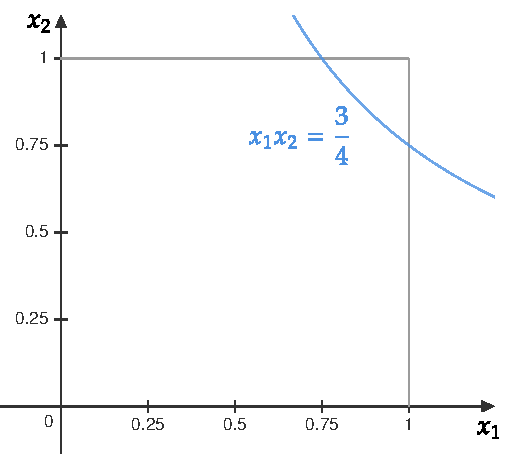
\includegraphics[width=0.9\linewidth]{RectangularHyperbola.pdf}
\end{minipage}

Now the significance level is obtained by evaluating the power function at the parameter point where the null hypothesis $H_0$ is true, that is at $\theta = 1$. Therefore, the significance level is
\begin{align*}
\alpha &= K(1) \\
& = \dfrac 1 4 + \dfrac 3 4 \log \dfrac 3 4 \\
& \approx 0.034.
\end{align*}
\end{Solution*}

\item Let $(X_1, X_2)$ be a random sample of size $2$ from the distribution having pdf $f(x; \theta) = \dfrac 1 \theta e^{-x/\theta}$, $x > 0$, where $\theta > 0$. We reject $H_0 \colon \theta = 2$ and accept $H_1 \colon \theta = 1$ if the observed value $(x_1, x_2)$ of the sample is such that
\begin{equation*}
\dfrac{f(x_1; 2) f(x_2; 2)}{f(x_1; 1) f(x_2; 1)} \le \dfrac 1 2.
\end{equation*}
Find the significance level of the test and the power of the test when $H_1$ is true.
\begin{Solution*}
The critical region is defined by
\begin{align*}
\dfrac{f(x_1; 2) f(x_2; 2)}{f(x_1; 1) f(x_2; 1)} & \le \dfrac 1 2 \iff \\
\dfrac 1 4 \times \dfrac{e^{-\frac{x_1 + x_2} 2}}{e^{-(x_1 + x_2)}} & \le \dfrac 1 2 \iff \\
e^{\frac {x_1 + x_2} 2} & \le 2 \iff\\
x_1 + x_2 & \le \log 4.
\end{align*}

Now, $g(x_1, x_2; \theta) = \dfrac 1 {\theta^2} e^{-\frac{x_1 + x_2}{\theta}}$, $x_1, x_2 > 0$.

The power function is\\
\begin{minipage}[h]{0.5\linewidth}
\begin{align*}
K(\theta) &= \dfrac 1 {\theta^2} \int_0^{\log 4} \int_0^{\log 4 - x_1} e^{-\frac{x_1 + x_2}{\theta}} \,dx_2 \,dx_1 \\
	&= \dfrac 1 \theta \int_0^{\log 4} e^{-\frac {x_1} \theta} \bqty{ 1 - e^{\frac{x_1 - \log 4}{\theta}} } \,dx_1 \\
	& = \dfrac 1 \theta \int_0^{\log 4} e^{-\frac {x_1} \theta} - 4^{- \frac 1 \theta} \,dx_1\\
	& = 1 - 4^{- \frac 1 \theta}  + 4^{- \frac 1 \theta} \log 4^{- \frac 1 \theta}.
\end{align*}
\end{minipage}\qquad
\begin{minipage}{0.4\linewidth}
\includegraphics[width=0.8\linewidth]{"x + y = log 4.pdf"}
\end{minipage}

Then the significance level is
\begin{align*}
\alpha & = K(2) \qquad [\because H_0 \colon \theta = 2]\\
	& =\dfrac 1 2 + \dfrac 1 2 \log \dfrac 1 2\\
	& \approx 0.15.
\end{align*}

$H_1$ is true when $\theta = 1$. Thus, the power of the test when $H_1$ is true is
\begin{align*}
K(1) = \dfrac 3 4 + \dfrac 1 4\log \dfrac 1 4 \approx 0.4. 
\end{align*}
\end{Solution*}

\item The life length of a tyre in miles, $X$, is normally distributed with mean $\theta$ and standard deviation $5000$. Past experience indicates that $\theta = 30,000$. The manufacturer claims that the tyres made by a new procedure have $\theta > 30,000$ and it is very likely that $\theta = 35,000$. Check the claim by testing $H_0 \colon \theta \le 30,000$ against $H_1 \colon \theta > 30,000$. Observe $n$ independent values of $X$, say $x_1, x_2, \ldots, x_n$ and reject $H_0$ if and only if $\overline x > c$. Determine $n$ and $c$ so that the power function $K(\theta)$ has values $K(30,000) = 0.01$ and $K(35,000) = 0.98$.
\begin{Solution*}
$K(\theta) = P[\overline X > c \mid \theta]$ (where $\overline X$ is the sample mean\footnote{
	Here we write $\overline X$ because it is a random variable, not the particular value $\overline x$ obtained after the experiment.
}).

Since $X \sim N(\theta, 5000^2)$, the sample mean $\overline X \sim N \pqty{\theta, \dfrac{5000^2}n}$. Therefore, $Z = \dfrac{\overline X - \theta}{5000/\sqrt n} \sim N(0, 1)$.
\begin{align*}
K(30,000) & = 0.01 \implies \\
P[\overline X > c \mid \theta = 30000]	& = 0.01 \implies \\
P\bqty{ Z > \dfrac{c - 30000}{5000/\sqrt n} } & = 0.01 \implies \\
P\bqty{ Z \le \dfrac{c - 30000}{5000/\sqrt n} } & = 0.99 \implies \\
\dfrac{c - 30000}{5000/\sqrt n} & = 2.33 \tag{1} \label{eq:3.1}
\end{align*}

\begin{align*}
P[\overline X > c \mid \theta = 35000] & = 0.98 \implies \\
P\bqty{ Z > \dfrac{c - 35000}{5000/\sqrt n} } & = 0.98 \implies \\
P\bqty{ Z \le \dfrac{c - 35000}{5000/\sqrt n} } & = 0.98 \implies \\
\dfrac{c - 35000}{5000/\sqrt n} & = 2.06 \tag{2} \label{eq:3.2}
\end{align*}

From \eqref{eq:3.1} and \eqref{eq:3.2}, $n = 19.2 \approx 19$ and $c = 32653.8$.
\end{Solution*}
\end{enumerate}

\subsection{Exercises}\label{subsec:Exercises1}
\begin{enumerate}
\item Let $X$ have a Poisson distribution with mean $\theta$. Test the simple hypothesis $H_0 \colon \theta = 0.5$ against the composite hypothesis $\theta < 0.5$ by using a sample $(X_1, \ldots, X_{12})$ of size $12$. Reject $H_0$ if and only if the observed value of $Y = X_1 + \cdots + X_{12} \le 2$. Find the powers $K(\frac 1 2)$, $K(\frac 1 3)$, $K(\frac 1 4)$, $K(\frac 1 6)$, and $K(\frac 1 {12})$. What is the significance level of the test?

\item Let $Y$ have a binomial distribution with parameters $n$ and $p$. We reject $H_0 \colon p = \frac 1 2$ and accept $H_1 \colon p > \frac 1 2$ if $Y \ge c$. Find $n$ and $c$ to give a power function $K(p)$ which is such that $K(\frac 1 2) = 0.1$ and $K(\frac 2 3) = 0.95$, approximately.

\item Let $X \sim U[0, \theta]$. Test $H_0 \colon \theta = 1$ against $H_1 \colon \theta = 2$ using a sample $(X_1, X_2)$ of size $2$, by rejecting $H_0$ if either $\overline X > 0.75$ or at least one of $X_1$ and $X_2$ is greater than $1$. Compute $K(1)$ and $K(2)$.
\end{enumerate}

\section{Chi-Square Tests}\label{sec:Chi-square}
In Section~\ref{sec:Intro}, we considered the problem of determining if a given coin was fair or biased. Now imagine that the same question is asked about a given six-sided die. Again, we can test the hypothesis that the die is fair, by throwing it $n$ times and observing the distribution of the resulting outcomes. Now, however, we have not two but six different classes into which the outcomes are divided\footnote{
	Recall that in the case of a coin, the two classes are number of heads and number of tails -- and given the total number of tosses, it is enough to specify just one of these, say, the number of heads obtained.
} -- namely the number of appearances of $1$, the number of appearances of $2$, \ldots, the number of appearances of $6$. Let these numbers be denoted by $x_1, x_2, \ldots, x_6$. We also have the probabilities $p_1, p_2, \ldots, p_6$ for the occurrence of the respective faces $1, 2, \ldots, 6$ of the die in each throw. In the case of a fair die, each of these would be $p_i = \frac 1 6$. Since $n$ is the total number of throws, we expect that each observed number $x_i$ should be more or less equal to $np_i$. For instance, if we throw the die $60$ times, then if the die is fair, each face should appear roughly $10$ times. Therefore the difference $x_i - np_i$ between the observed and expected number of appearances is a measure of how \emph{false} our hypothesis is likely to be. Therefore we need to design a test that uses these deviations to estimate the probability of the truth or falsehood of the hypothesis.

Firstly, observe that $x_6 = n - (x_1 + \cdots + x_5)$, so that we only need to consider $x_1, \ldots, x_5$. The sample $(X_1, X_2, \ldots, X_5)$ has what is known as the multinomial distribution\footnote{
	The multinomial distribution is a generalisation of the binomial distribution -- the multinomial distribution with only two parameters $n$ and $p_1$ is exactly $B(n, p_1)$.
} with parameters $n, p_1, \ldots, p_5$. Then if we define
\begin{align*}
Q_5 ={} &  \dfrac{(X_1 - np_1)^2}{np_1} + \dfrac{(X_2 - np_2)^2}{np_2} + \dfrac{(X_3 - np_3)^2}{np_3} + {}\\
 & \dfrac{(X_4 - np_4)^2}{np_4} + \dfrac{(X_5 - np_5)^2}{np_5} + \dfrac{(X_6 - np_6)^2}{np_6},
\end{align*}
$Q_5 \sim \chi^2_5$ approximately for large $n$ (i.e., in the limiting case where $n \to \infty$).

Now the test is as follows. Select a value $c$, and reject the hypothesis that the die is fair if $Q_5 \ge c$. What should be the ideal value of $c$? That depends on the significance level of the test. What we can do therefore, is to \emph{set} a desired significance level $\alpha$ and select $c$ such that $P(Q_5 \ge c) = \alpha$. This value of $c$ can be obtained from the chi-square.

The chi-square test in general can therefore be described as follows. Given $k$ classes $C_1, C_2, \ldots, C_k$, to test the hypothesis $H_0$ that the probability distribution of these classes is $p_1, p_2, \ldots, p_k$ respectively (where $p_1 + \cdots + p_k = 1$), we conduct $n$ trials and observe the frequencies $X_1, X_2, \ldots, X_k$ of the respective classes (so that $X_1 + X_2 + \cdots + X_k = n$). Now define
\begin{equation*}
Q_{k - 1} = \sum_{i=1}^{k} \dfrac{(X_i - np_i)^2}{np_i}.
\end{equation*}
Then the chi-square test with significance level $\alpha$ is to reject $H_0$ if $Q_{k - 1} \ge c$, where $c$ is the value such that $P[Q_{k - 1} \ge c] = \alpha$. Common values of $\alpha$ are $0.05$ and $0.01$, written as $5\%$ and $1\%$ respectively.

\subsection{Solved Problems}\label{subsec:SolvedProblems2}
\begin{enumerate}
\item A six-sided die is thrown $60$ times and the observed frequencies of the faces $1, 2, \ldots, 6$ are $13, 19, 11, 8, 5, 4$ respectively. Test whether the die is fair, at $5\%$ level of significance.
\begin{Solution*}
Here, we have number of classes $k = 6$, and theoretical probabilities $p_1 = p_2 = \cdots = p_6 = \frac 1 6$ (since a fair die must have equally likely outcomes), so that $np_i = 10$, $i = 1, 2, \ldots, 10$. Then,
\begin{align*}
Q_5 & = \sum_{i = 1}^5 \dfrac{(x_i - np_i)^2}{np_i} \\
	& = \dfrac{(13- 10)^2}{10} + \dfrac{(19 - 10)^2}{10} + \dfrac{(11 - 10)^2}{10} + \dfrac{(8 - 10)^2}{10} + \dfrac{(5 - 10)^2}{10} + \dfrac{(4 - 10)^2}{10} \\
	& = 15.6.
\end{align*}

But $\chi^2_5 = 11.1$ at $5\%$ level of significance. Thus, $Q_5 > \chi^2_5$, which means that \textbf{we reject the hypothesis that the die is fair}.
\end{Solution*}

\item The Mendelian theory of genetics of crossing two types of peas states that the probabilities of classification of the four resulting types are $\frac 9 {16}$, $\frac 3 {16}$, $\frac 3 {16}$, and $\frac 1 {16}$ respectively. If, from $160$ independent observations, the observed frequencies of these classifications are $86, 35, 26, 13$ respectively, test whether the data is consistent with the theory with $\alpha = 0.01$.
\begin{Solution*}
Here, $k = 4$, $n = 160$, and $np_1 = 90$, $np_2 = 30$, $np_3 = 30$, $np_4 = 10$. Therefore,
\begin{align*}
Q_3 & = \dfrac{(86 - 90)^2}{90} + \dfrac{(35 - 30)^2}{30} + \dfrac{(26 - 30)^2}{30} + \dfrac{(13 - 10)^2}{10}\\
	& = 2.44 < 11.345 = \chi^2_3
\end{align*}
at $1\%$ level of significance (since $\alpha = 0.01$).

Thus, we \textbf{accept} the hypothesis -- i.e, the data is consistent with Mendelian theory.
\end{Solution*}
\end{enumerate}

\subsection{Exercises}\label{subsec:Exercises2}
\begin{enumerate}
\item The table below lists the observed results of $n = 120$ independent throws of a die.

\begin{tabular}{|r||c|c|c|c|c|c|}
	\hline
	Face & 1 & 2 & 3 & 4 & 5 & 6\\
	\hline
	Frequency & $a$ & $20$ & $20$ & $20$ & $20$ & $40 - a$\\
	\hline
\end{tabular}

For what values of $a$ would the hypothesis that the die is unbiased be rejected at $0.025$ level of significance in a chi-square test?

\item A manufacturer of lightbulbs claims that the lightbulbs produced fall into five categories A, B, C, D, and E by quality, from highest to lowest, and that the percentages of lightbulbs in these five categories are $15$, $25$, $35$, $20$, and $5$ respectively. A contractor who purchases a large number of the lightbulbs tests the claim by taking a random sample of $30$ lightbulbs and observes that the numbers of lightbulbs that fall in the categories A, B, C, D, and E are $3$, $6$, $9$, $7$, and $5$ respectively. Test whether the manufacturer is speaking the truth, using a chi-square test
\begin{enumerate}[label=(\roman*)]
\item at $5\%$ significance level;
\item at $1\%$ significance level.
\end{enumerate}
\end{enumerate}

\begin{appendices}
\section{Critical Values of $\chi^2$}
\begin{equation*}
\arraycolsep=15pt\def\arraystretch{1.2}
\begin{array}{crrr}
\hline
& \multicolumn{3}{c}{\text{Significance level}}\\
\text{D.f} & 5\% & 1\% & 0.1\% \\
\hline
1 & 3.841  &   6.635  & 10.828 \\
2 & 5.991  &   9.210  & 13.816 \\
3 & 7.815  &   11.345 &  16.266 \\
4 & 9.488  &   13.277 &  18.467 \\
5 & 11.070 &   15.086 &  20.515 \\
6 & 12.592 &   16.812 &  22.458 \\
7 & 14.067 &   18.475 &  24.322 \\
8 & 15.507 &   20.090 &  26.124 \\
9 & 16.919 &   21.666 &  27.877 \\
10 & 18.307 &  23.209 &  29.588 \\
\hline
\end{array}
\end{equation*}
\end{appendices}
\end{document}